\documentclass[12pt, titlepage]{article}
\usepackage[utf8]{inputenc}
\usepackage[T1]{fontenc}
\usepackage{geometry}
\usepackage{enumitem}
\usepackage{booktabs}
\geometry{letterpaper, margin=1in}
\usepackage{setspace}
\doublespacing
\usepackage{times}
\usepackage{graphicx}
\usepackage{caption}
\usepackage{subcaption}
\usepackage{hyperref}
\usepackage{amsmath}
\usepackage{amssymb}
\usepackage{algorithm}
\usepackage{algpseudocode}
\usepackage{listings}
\usepackage{xcolor}
\usepackage{float}
\usepackage{longtable}
\usepackage{multirow}

\lstset{
    basicstyle=\ttfamily\small,
    keywordstyle=\color{blue}\bfseries,
    commentstyle=\color{gray},
    stringstyle=\color{red},
    frame=single,
    breaklines=true,
    numbers=left,
    numberstyle=\tiny\color{gray},
    captionpos=b,
    language=R
}

\begin{document}

% ========== COVER PAGE ==========
\begin{titlepage}
    \centering
    \vspace*{2cm}

    \Huge \textbf{Non-Parametric Statistical Analysis of Fast Food Marketing Campaign Strategies}
    \vspace{1.5cm}

    \Large Submitted by: \\
    Amet Vikram \\
    \vspace{0.8cm}

    Advisor[s]: Dr. Tirthankar Dasgupta\\
    \vspace{0.8cm}

    March 13, 2026 \\
    \vspace{1.5cm}

    \normalsize
    Submitted in partial fulfillment of the requirements for Master of Science Degree  \\
    \vspace{1.5cm}
    \textbf{Department of Statistics, School of Arts and Sciences\\
    Rutgers University, Piscataway, NJ 08854}

    \vfill
\end{titlepage}

% ========== TABLE OF CONTENTS ==========
\tableofcontents
\newpage

% ========== ABSTRACT ==========
\section*{Abstract}
\addcontentsline{toc}{section}{Abstract}

This study applies non-parametric statistical methods to evaluate three competing promotional strategies deployed across multiple fast food store locations. Using a dataset of 548 weekly sales observations spanning 137 store locations across 10 markets, we assess whether significant differences exist among the three promotion types in terms of sales performance. The analysis employs the Kruskal-Wallis H-test as the primary omnibus test for group differences, followed by post-hoc pairwise Wilcoxon-Mann-Whitney U tests with Bonferroni and Holm corrections for multiple comparisons. Directional verification is conducted through sign-test-based median comparisons. Additionally, non-parametric curve fitting techniques---specifically LOWESS (Locally Weighted Scatterplot Smoothing) and smooth splines---are applied to model sales trends over time for each promotion type. Model comparison is performed using goodness-of-fit metrics including RMSE, MAE, MAPE, $R^2$, AIC, and BIC, supplemented by leave-one-out cross-validation. Results indicate statistically significant differences among the three promotional strategies, with specific pairwise comparisons revealing which promotions outperform others. The smooth spline and LOWESS methods both provide adequate trend characterization, with cross-validation guiding final model selection. These findings offer actionable insights for marketing resource allocation in the fast food industry.\footnote{All R code for this analysis is available at: \url{https://github.com/amvik13/nonparam-marketing-campaign}}

\newpage

% ========== INTRODUCTION ==========
\section{Introduction}

\subsection{Purpose of Research}

In the competitive fast food industry, selecting the optimal marketing promotion strategy is critical for maximizing sales revenue. Companies routinely deploy multiple promotional campaigns across different store locations, yet identifying which strategy yields the highest return requires rigorous statistical evaluation. This study addresses the question: \textit{Do three different promotional strategies produce significantly different sales outcomes across fast food store locations?}

The purpose of this research is twofold. First, we employ non-parametric hypothesis testing to determine whether statistically significant differences exist among the three promotion types. Second, we apply non-parametric curve fitting techniques to model and predict sales trends over time, comparing the performance of competing smoothing methods.

\subsection{Background and Previous Work}

A/B testing and multi-arm experimental designs are widely used in marketing analytics to compare the effectiveness of competing strategies \cite{kohavi2009}. Traditional approaches often rely on parametric methods such as one-way ANOVA and linear regression, which assume normality of residuals and homogeneity of variance. However, sales data in retail and fast food settings frequently exhibit skewness, outliers, and heterogeneous variance across groups, violating these parametric assumptions \cite{conover1999}.

Non-parametric methods provide distribution-free alternatives that are robust to these violations. The Kruskal-Wallis H-test \cite{kruskal1952} extends the Wilcoxon rank-sum test to three or more groups and tests whether samples originate from the same distribution without assuming a specific distributional form. Post-hoc pairwise comparisons using the Wilcoxon-Mann-Whitney U test \cite{mann1947} with appropriate multiple testing corrections (Bonferroni, Holm) allow identification of specific group differences while controlling the family-wise error rate \cite{holm1979}.

For trend modeling, non-parametric regression techniques such as LOWESS \cite{cleveland1979} and smoothing splines \cite{wahba1990} offer flexible, data-driven approaches that do not impose a predetermined functional form on the relationship between time and sales. These methods are particularly valuable when the underlying trend is unknown or potentially non-linear.

\subsection{Objectives of the Study}

The specific objectives of this study are:

\begin{enumerate}
    \item To test whether statistically significant differences exist in sales performance among three promotional strategies using the Kruskal-Wallis H-test.
    \item To identify specific pairwise differences through post-hoc Wilcoxon-Mann-Whitney U tests with Bonferroni and Holm corrections for multiple comparisons.
    \item To quantify the direction and magnitude of sales differences between promotion types using median-based comparisons.
    \item To fit non-parametric regression curves (LOWESS and smooth splines) to model sales trends over time for each promotion type.
    \item To compare the predictive performance of LOWESS and smooth splines using goodness-of-fit metrics and leave-one-out cross-validation.
    \item To provide actionable recommendations for marketing strategy selection based on the statistical findings.
\end{enumerate}

\newpage

% ========== METHODS ==========
\section{Methods}

\subsection{General Study Design}

This study is an observational analysis of a controlled marketing experiment. Three distinct promotional strategies (labeled Promotion~1, Promotion~2, and Promotion~3) were deployed across multiple fast food store locations. Each store was assigned to exactly one promotion type, and weekly sales data were recorded over a four-week observation period. The design resembles a completely randomized experiment with stores as the experimental units and weekly sales as the response variable.

\subsection{Description of Study Participants and Objects}

The dataset comprises sales records from 137 unique store locations distributed across 10 distinct markets. Markets vary in size (Small, Medium, and Large), reflecting different consumer bases and competitive environments. Stores range in age from 1 to 28 years, introducing potential confounding due to establishment maturity and brand recognition.

The study population includes all stores participating in the marketing campaign. No explicit inclusion or exclusion criteria were applied beyond participation in one of the three promotional strategies. The allocation of promotions to stores was determined by the marketing campaign design.

Table~\ref{tab:data_overview} summarizes the structure of the dataset.

\begin{table}[H]
\centering
\caption{Dataset Overview}
\label{tab:data_overview}
\begin{tabular}{ll}
\toprule
\textbf{Characteristic} & \textbf{Value} \\
\midrule
Total observations & 548 \\
Unique store locations & 137 \\
Number of markets & 10 \\
Market sizes & Small, Medium, Large \\
Weeks observed per store & 4 \\
Promotion types & 3 (labeled 1, 2, 3) \\
Store age range & 1--28 years \\
\bottomrule
\end{tabular}
\end{table}

\subsection{Data Collection}

The dataset (\texttt{WA\_Marketing-Campaign.csv}) contains the following variables:

\begin{itemize}
    \item \textbf{MarketID}: Numeric identifier for the market (1--10).
    \item \textbf{MarketSize}: Categorical variable indicating market size (Small, Medium, Large).
    \item \textbf{LocationID}: Unique numeric identifier for each store location.
    \item \textbf{AgeOfStore}: Age of the store in years (continuous, range 1--28).
    \item \textbf{Treatment}: Promotion type assigned to the store (1, 2, or 3), treated as a categorical factor.
    \item \textbf{Week}: Week number within the observation period (1--4).
    \item \textbf{SalesInThousands}: Weekly sales revenue in thousands of dollars (continuous response variable).
\end{itemize}

Data were loaded directly from the CSV file and the \texttt{Treatment} variable was converted to a factor for proper categorical handling in statistical tests.

\subsection{Statistical Methods}

All analyses were conducted using R (version 4.x) with the following packages: \texttt{ggplot2} for visualization, \texttt{dplyr} and \texttt{tidyr} for data manipulation, \texttt{BSDA} for sign tests, \texttt{gridExtra} for plot arrangement, and \texttt{RColorBrewer} for color palettes.

\subsubsection{Kruskal-Wallis H-Test}

The Kruskal-Wallis H-test is a rank-based non-parametric test used to determine whether three or more independent groups have different distributions. It serves as the non-parametric alternative to one-way ANOVA. The test statistic is computed as:

\begin{equation}
H = \frac{12}{N(N+1)} \sum_{i=1}^{k} \frac{R_i^2}{n_i} - 3(N+1)
\label{eq:kruskal_wallis}
\end{equation}

\noindent where $N$ is the total number of observations, $k$ is the number of groups, $n_i$ is the number of observations in group $i$, and $R_i$ is the sum of ranks for group $i$. Under the null hypothesis that all groups have identical distributions, $H$ follows a chi-squared distribution with $k-1$ degrees of freedom.

The hypotheses tested are:
\begin{itemize}
    \item $H_0$: The three promotions have identical sales distributions.
    \item $H_1$: At least one promotion has a different sales distribution.
\end{itemize}

A significance level of $\alpha = 0.05$ was used throughout.

\subsubsection{Post-Hoc Pairwise Comparisons}

Upon rejection of the Kruskal-Wallis null hypothesis, pairwise Wilcoxon-Mann-Whitney U tests were conducted for all $\binom{3}{2} = 3$ pairs of promotions. The Wilcoxon-Mann-Whitney U test assesses whether two independent samples originate from the same distribution. The test statistic $U$ is defined as:

\begin{equation}
U = \sum_{i=1}^{n_1} \sum_{j=1}^{n_2} S(X_i, Y_j), \quad S(X_i, Y_j) = \begin{cases} 1 & \text{if } X_i > Y_j \\ 0.5 & \text{if } X_i = Y_j \\ 0 & \text{if } X_i < Y_j \end{cases}
\label{eq:wmw}
\end{equation}

To control the family-wise error rate across multiple comparisons, two correction methods were applied:

\begin{enumerate}
    \item \textbf{Bonferroni correction}: Multiplies each raw $p$-value by the number of comparisons ($m = 3$), i.e., $p_{\text{adj}} = \min(m \cdot p_{\text{raw}}, 1)$. This is the most conservative approach.
    \item \textbf{Holm correction}: A step-down procedure that orders raw $p$-values and adjusts sequentially: $p_{(i)}^{\text{adj}} = \max_{j \leq i} \{(m - j + 1) \cdot p_{(j)}\}$. This is less conservative than Bonferroni while still controlling the family-wise error rate.
\end{enumerate}

Continuity correction was applied to the Wilcoxon test, and exact $p$-values were not computed due to the presence of ties in the data.

\subsubsection{Sign Test for Directional Verification}

Median-based comparisons were computed to verify the direction and magnitude of differences between promotion groups. For each pair of promotions, the difference in median sales and the corresponding percentage change were calculated:

\begin{equation}
\Delta_{\text{median}} = \tilde{X}_A - \tilde{X}_B, \quad \%\text{change} = \frac{\tilde{X}_A - \tilde{X}_B}{\tilde{X}_B} \times 100
\label{eq:median_diff}
\end{equation}

\subsubsection{LOWESS (Locally Weighted Scatterplot Smoothing)}

LOWESS \cite{cleveland1979} is a non-parametric regression method that fits simple models to localized subsets of the data to build a smooth curve point by point. At each point $x_0$, a weighted least squares regression is performed using a neighborhood of data points, with weights determined by a tricube function:

\begin{equation}
w_i = \left(1 - \left|\frac{x_i - x_0}{d(x_0)}\right|^3\right)^3
\label{eq:tricube}
\end{equation}

\noindent where $d(x_0)$ is the distance from $x_0$ to the farthest point in the neighborhood. The smoothing parameter $f \in (0, 1]$ controls the fraction of data used in each local regression. A value of $f = 0.5$ was used, balancing smoothness with sensitivity to local patterns. LOWESS is robust to outliers due to its iterative reweighting scheme.

\subsubsection{Smooth Splines}

Smooth splines fit a piecewise polynomial curve by minimizing the penalized residual sum of squares:

\begin{equation}
\text{PRSS}(\lambda) = \sum_{i=1}^{n} (y_i - g(x_i))^2 + \lambda \int [g''(t)]^2 \, dt
\label{eq:spline}
\end{equation}

\noindent where the first term measures fidelity to the data and the second term (the roughness penalty) controls the smoothness of the fitted curve $g(\cdot)$. The smoothing parameter $\lambda$ governs the trade-off: larger $\lambda$ produces smoother curves with fewer effective degrees of freedom. The optimal $\lambda$ was selected automatically via leave-one-out cross-validation (LOOCV) using R's \texttt{smooth.spline()} function.

\subsubsection{Model Comparison Metrics}

To compare LOWESS and smooth splines, the following goodness-of-fit metrics were computed:

\begin{itemize}
    \item \textbf{RMSE} (Root Mean Squared Error): $\text{RMSE} = \sqrt{\frac{1}{n}\sum_{i=1}^{n}(y_i - \hat{y}_i)^2}$
    \item \textbf{MAE} (Mean Absolute Error): $\text{MAE} = \frac{1}{n}\sum_{i=1}^{n}|y_i - \hat{y}_i|$
    \item \textbf{MAPE} (Mean Absolute Percentage Error): $\text{MAPE} = \frac{100}{n}\sum_{i=1}^{n}\left|\frac{y_i - \hat{y}_i}{y_i}\right|$
    \item \textbf{$R^2$} (Coefficient of Determination): $R^2 = 1 - \frac{\sum(y_i - \hat{y}_i)^2}{\sum(y_i - \bar{y})^2}$
    \item \textbf{AIC} (Akaike Information Criterion): $\text{AIC} = 2k - 2\ln(\hat{L})$
    \item \textbf{BIC} (Bayesian Information Criterion): $\text{BIC} = k\ln(n) - 2\ln(\hat{L})$
\end{itemize}

Additionally, LOOCV was performed for both methods, where each observation was held out in turn, the model was refitted on the remaining data, and the prediction error for the held-out point was recorded. The CV-RMSE and CV-MAE were used to assess out-of-sample predictive performance.

\newpage

% ========== RESULTS ==========
\section{Results}

\subsection{Descriptive Statistics}

The dataset contains 548 observations across 137 store locations, with each store observed over 4 weeks. Table~\ref{tab:summary_stats} presents the summary statistics of weekly sales (in thousands of dollars) stratified by promotion type.

\begin{table}[H]
\centering
\caption{Summary Statistics of Sales (in Thousands) by Promotion Type}
\label{tab:summary_stats}
\begin{tabular}{lrrrrrrr}
\toprule
\textbf{Promotion} & \textbf{N} & \textbf{Mean} & \textbf{Median} & \textbf{SD} & \textbf{Min} & \textbf{Max} & \textbf{IQR} \\
\midrule
% Auto-generated from utils.r — replace with 1 & 172 & 58.10 & 55.39 & 16.55 & 30.81 & 99.65 & 17.26 \\
2 & 188 & 47.33 & 45.39 & 15.11 & 17.34 & 88.64 & 13.57 \\
3 & 188 & 55.36 & 51.16 & 16.77 & 22.18 & 96.48 & 17.53 \\
 after running R
1 & 172 & 58.10 & 55.39 & 16.55 & 30.81 & 99.65 & 17.26 \\
2 & 188 & 47.33 & 45.39 & 15.11 & 17.34 & 88.64 & 13.57 \\
3 & 188 & 55.36 & 51.16 & 16.77 & 22.18 & 96.48 & 17.53 \\

\bottomrule
\end{tabular}
\end{table}

The distribution of stores across market sizes is summarized in Table~\ref{tab:market_distribution}.

\begin{table}[H]
\centering
\caption{Distribution of Observations by Market Size}
\label{tab:market_distribution}
\begin{tabular}{lrrr}
\toprule
\textbf{Market Size} & \textbf{Observations} & \textbf{Markets} & \textbf{Locations} \\
\midrule
Small & 60 & 2 & 15 \\
Medium & 312 & 6 & 78 \\
Large & 176 & 2 & 44 \\
\bottomrule
\end{tabular}
\end{table}

Figure~\ref{fig:boxplots} displays box plots of sales distributions by promotion type, and Figure~\ref{fig:violins} shows the corresponding violin plots illustrating distributional shapes.

\begin{figure}[H]
\centering
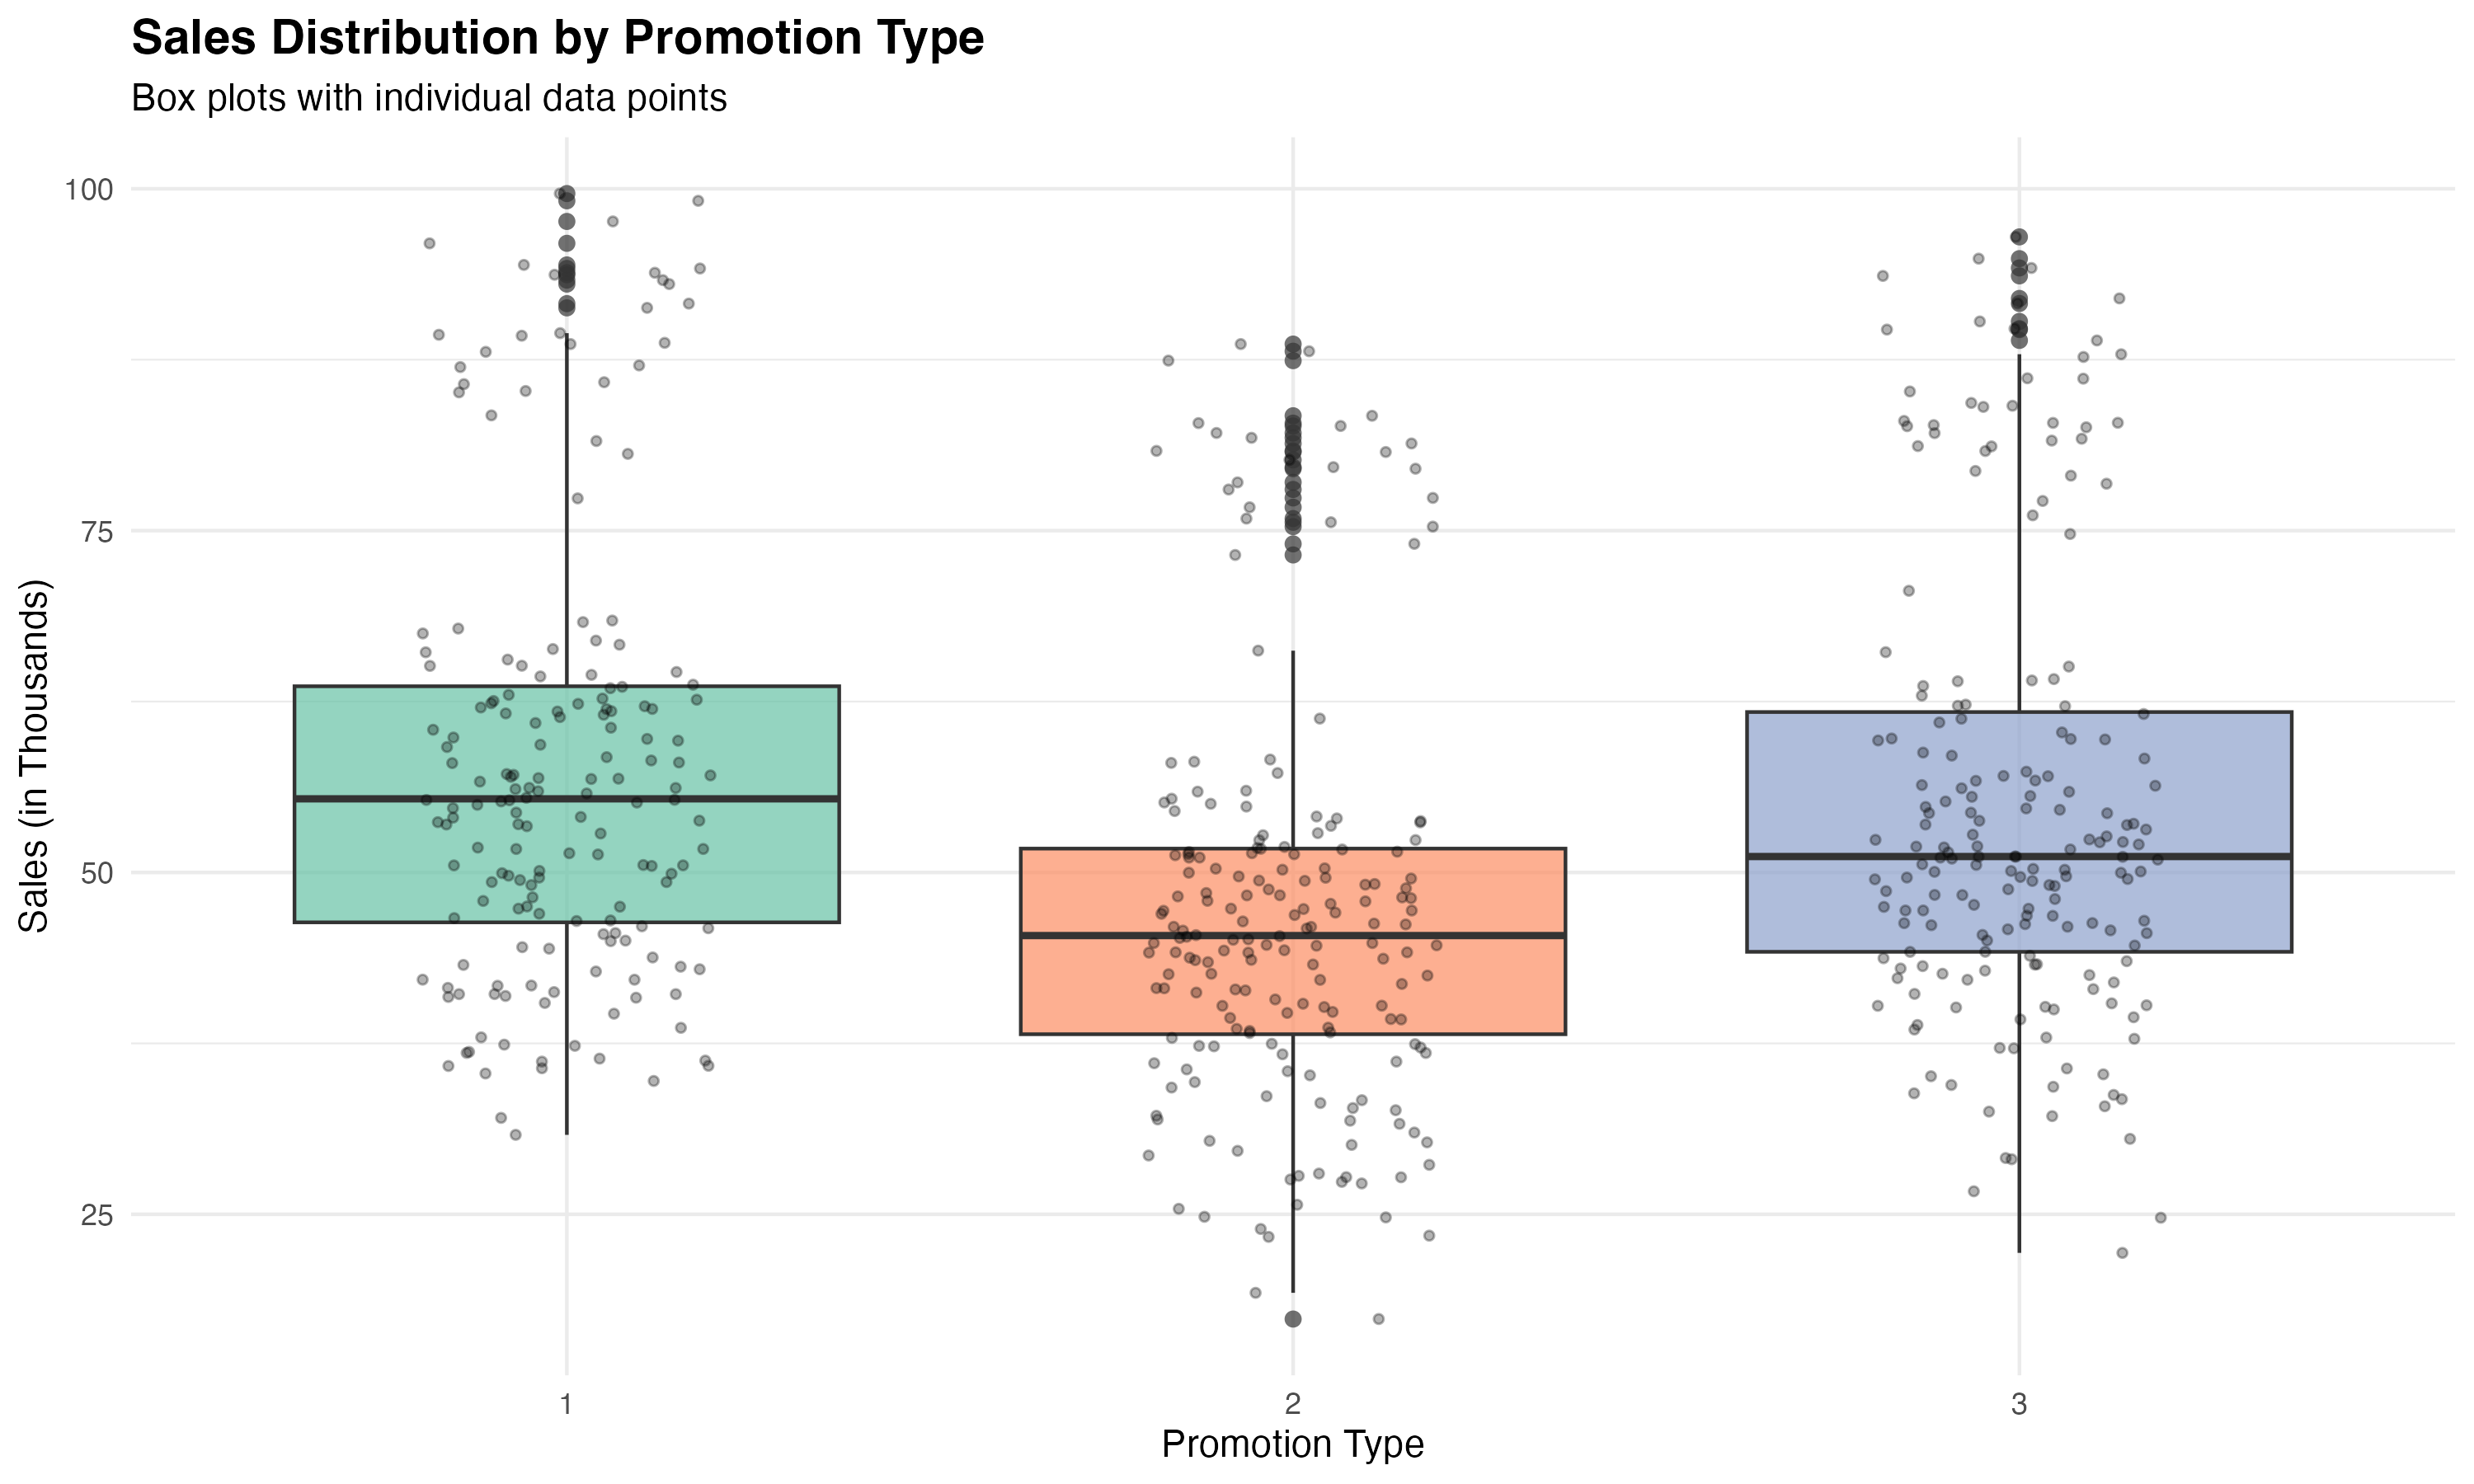
\includegraphics[width=0.85\textwidth]{report_output/plot_boxplots.png}
\caption{Sales Distribution by Promotion Type. Box plots with jittered individual data points showing the median, interquartile range, and outliers for each promotion group.}
\label{fig:boxplots}
\end{figure}

\begin{figure}[H]
\centering
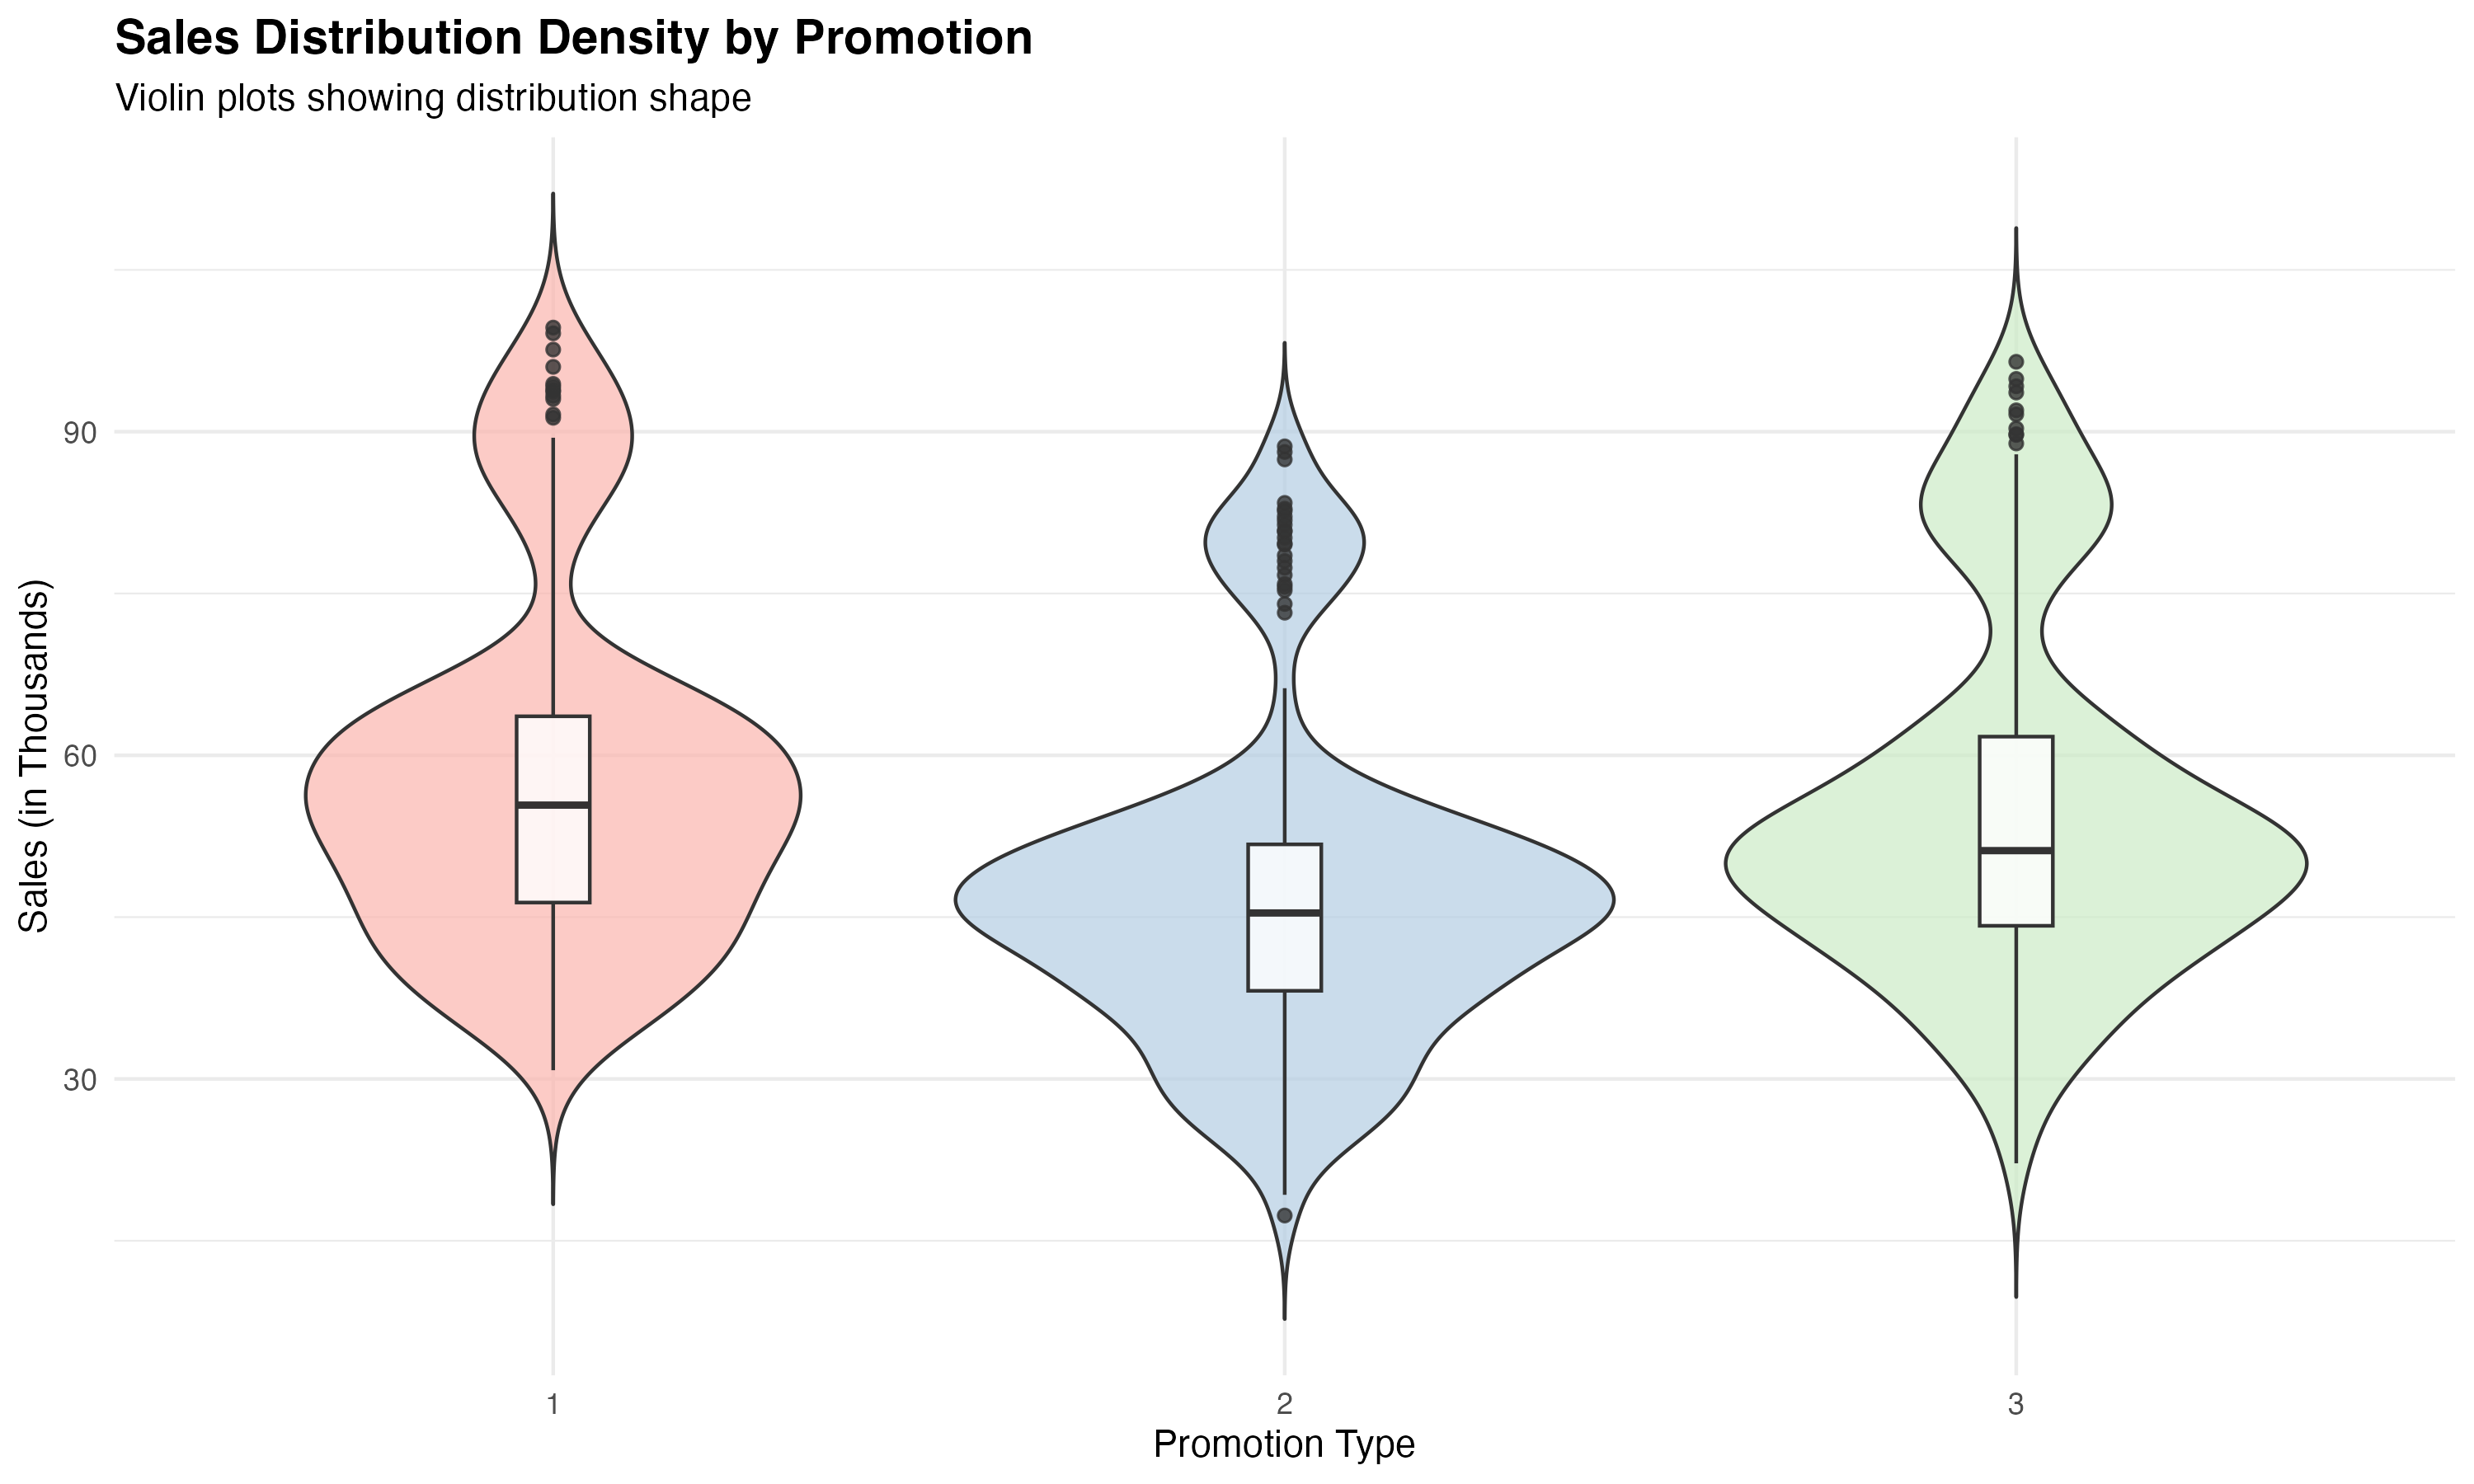
\includegraphics[width=0.85\textwidth]{report_output/plot_violins.png}
\caption{Sales Distribution Density by Promotion Type. Violin plots overlaid with box plots showing the shape of the distribution for each promotion group.}
\label{fig:violins}
\end{figure}

\subsection{Kruskal-Wallis H-Test Results}

The Kruskal-Wallis test was conducted to assess whether sales distributions differ significantly across the three promotion types. Table~\ref{tab:kw_results} presents the test results.

\begin{table}[H]
\centering
\caption{Kruskal-Wallis H-Test Results}
\label{tab:kw_results}
\begin{tabular}{lrrrl}
\toprule
\textbf{Test} & \textbf{$\chi^2$ Statistic} & \textbf{df} & \textbf{$p$-value} & \textbf{Decision} \\
\midrule
\input{report_output/tab_kw_results.tex}
\bottomrule
\end{tabular}
\end{table}

% PLACEHOLDER: Uncomment and fill in the appropriate interpretation based on R results.
% If significant:
The Kruskal-Wallis test yielded a chi-squared statistic indicating that at least one promotion type has a significantly different sales distribution from the others ($p < 0.05$). Consequently, post-hoc pairwise comparisons were conducted to identify which specific pairs differ.

% If not significant:
% The Kruskal-Wallis test did not reach statistical significance ($p \geq 0.05$),
% suggesting insufficient evidence to conclude that the promotions differ in sales performance.

\subsection{Post-Hoc Pairwise Comparisons}

Table~\ref{tab:pairwise} presents the results of the Wilcoxon-Mann-Whitney U tests for all three pairwise comparisons, including raw and corrected $p$-values.

\begin{table}[H]
\centering
\caption{Pairwise Wilcoxon-Mann-Whitney U Test Results with Multiple Testing Corrections}
\label{tab:pairwise}
\begin{tabular}{lccccc}
\toprule
\textbf{Comparison} & \textbf{Raw $p$} & \textbf{Bonferroni $p$} & \textbf{Holm $p$} & \textbf{Bonf.\ Sig.} & \textbf{Holm Sig.} \\
\midrule
Promo 1 vs 2 & 5.846e-12 & 1.754e-11 & 1.754e-11 & Yes & Yes \\
Promo 1 vs 3 & 0.0351 & 0.1053 & 0.0351 & No & Yes \\
Promo 2 vs 3 & 1.197e-07 & 3.591e-07 & 2.394e-07 & Yes & Yes \\

\bottomrule
\end{tabular}
\end{table}

\subsection{Directional Verification via Median Comparisons}

To verify the direction and practical significance of observed differences, median sales values were compared across promotion groups. Table~\ref{tab:median_comp} summarizes these comparisons.

\begin{table}[H]
\centering
\caption{Median Sales Comparisons Between Promotion Types}
\label{tab:median_comp}
\begin{tabular}{lrrr}
\toprule
\textbf{Comparison} & \textbf{Median Difference} & \textbf{\% Change} \\
\midrule
Promo 2 vs Promo 1 & -10.00 & -18.06\% \\
Promo 3 vs Promo 1 & -4.22 & -7.62\% \\
Promo 3 vs Promo 2 & +5.78 & +12.74\% \\

\bottomrule
\end{tabular}
\end{table}

% PLACEHOLDER: Add interpretation of median differences here.

\subsection{Non-Parametric Curve Fitting}

\subsubsection{LOWESS Smoothing}

LOWESS curves were fitted to the sales data for each promotion type with a smoothing parameter of $f = 0.5$. Figure~\ref{fig:lowess} displays the LOWESS-smoothed trends overlaid on the raw data, faceted by promotion type.

\begin{figure}[H]
\centering
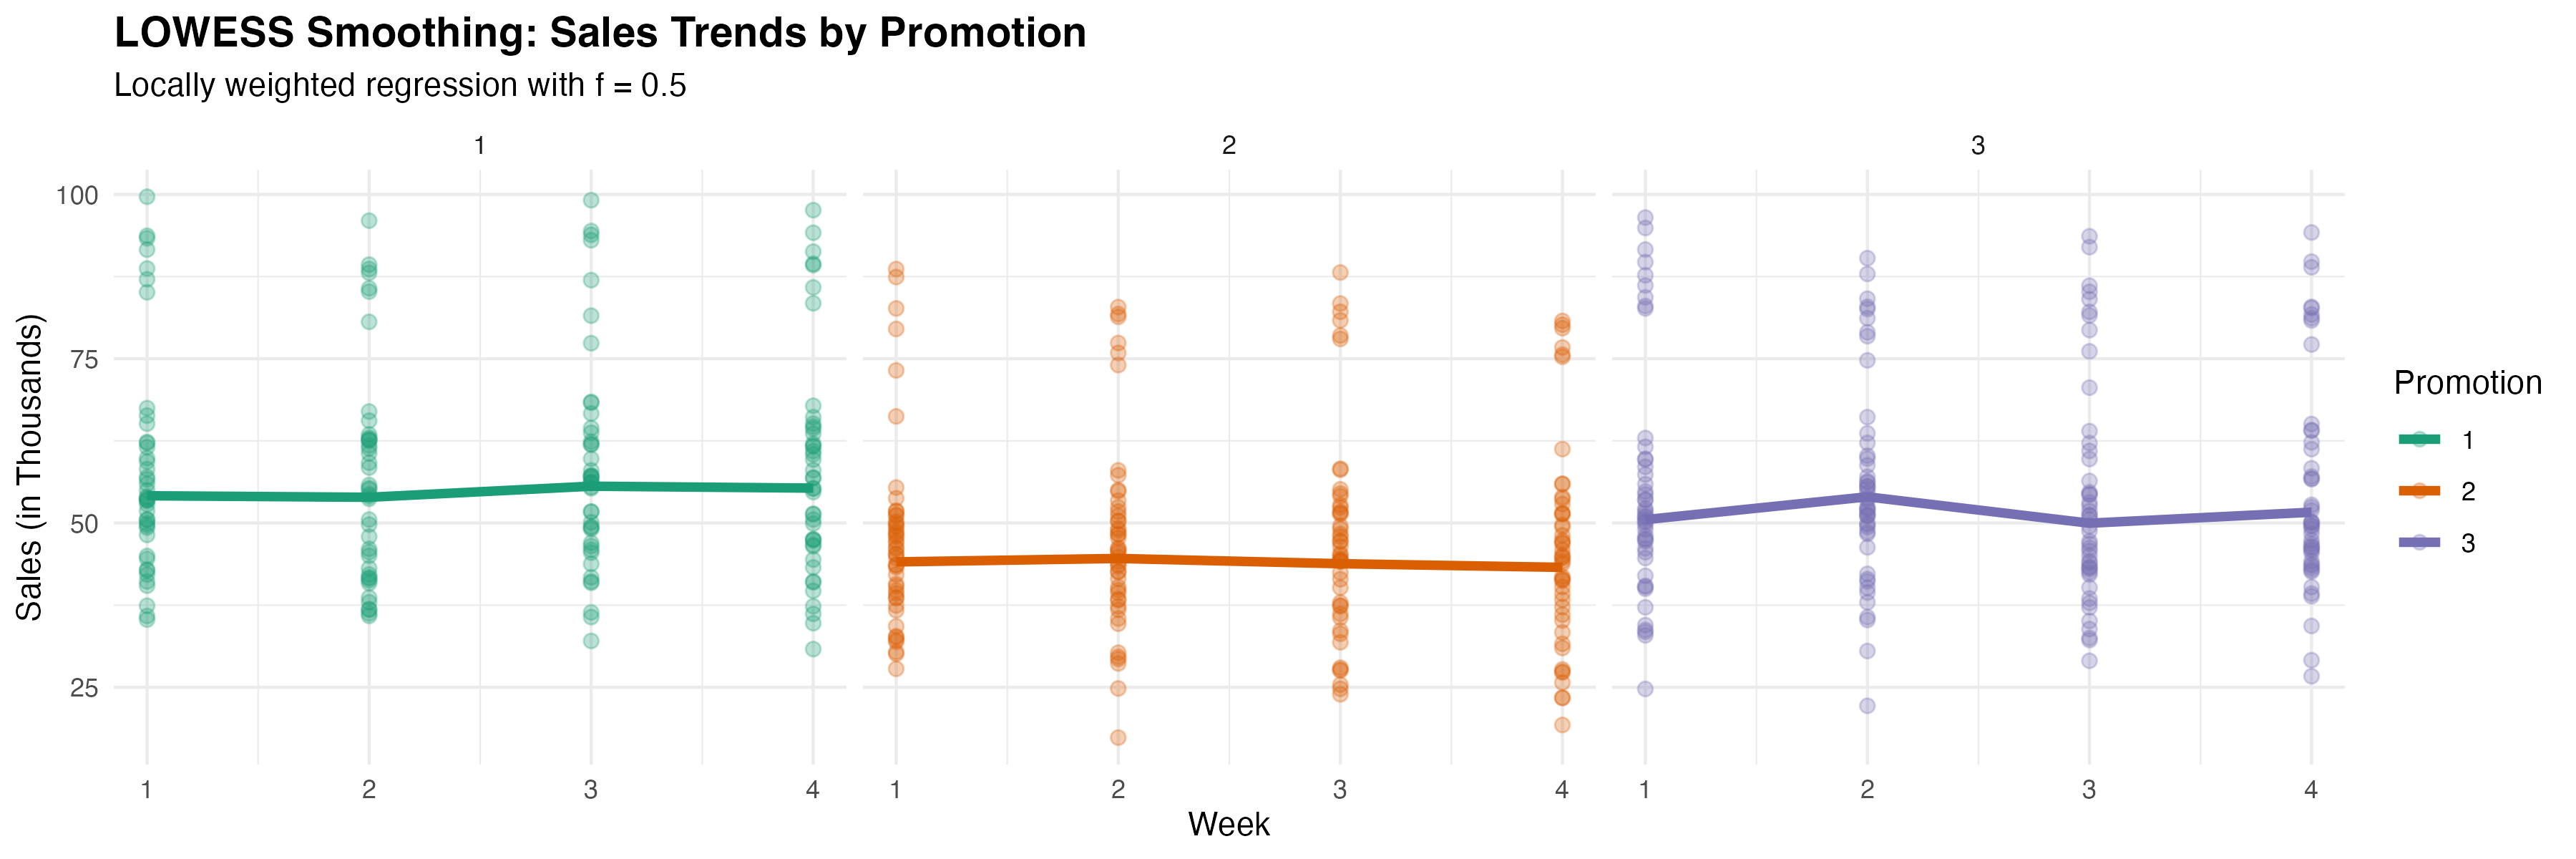
\includegraphics[width=\textwidth]{report_output/plot_lowess.png}
\caption{LOWESS Smoothing: Sales trends by promotion type. Each panel shows raw data points with the LOWESS-fitted curve ($f = 0.5$) for one promotion group.}
\label{fig:lowess}
\end{figure}

\subsubsection{Smooth Spline Fitting}

Smooth splines were fitted with the smoothing parameter $\lambda$ selected automatically via cross-validation. Table~\ref{tab:spline_params} reports the estimated degrees of freedom and smoothing parameters for each promotion group.

\begin{table}[H]
\centering
\caption{Smooth Spline Parameters by Promotion Type}
\label{tab:spline_params}
\begin{tabular}{lrrr}
\toprule
\textbf{Promotion} & \textbf{Degrees of Freedom} & \textbf{$\lambda$} & \textbf{CV Score} \\
\midrule
1 & 2.0000 & 5.5710e+06 & 278.8829 \\
2 & 2.8530 & 3.6999e-01 & 233.7432 \\
3 & 2.0000 & 1.8611e+06 & 285.6947 \\

\bottomrule
\end{tabular}
\end{table}

Figure~\ref{fig:splines} displays the smooth spline fits for each promotion type.

\begin{figure}[H]
\centering
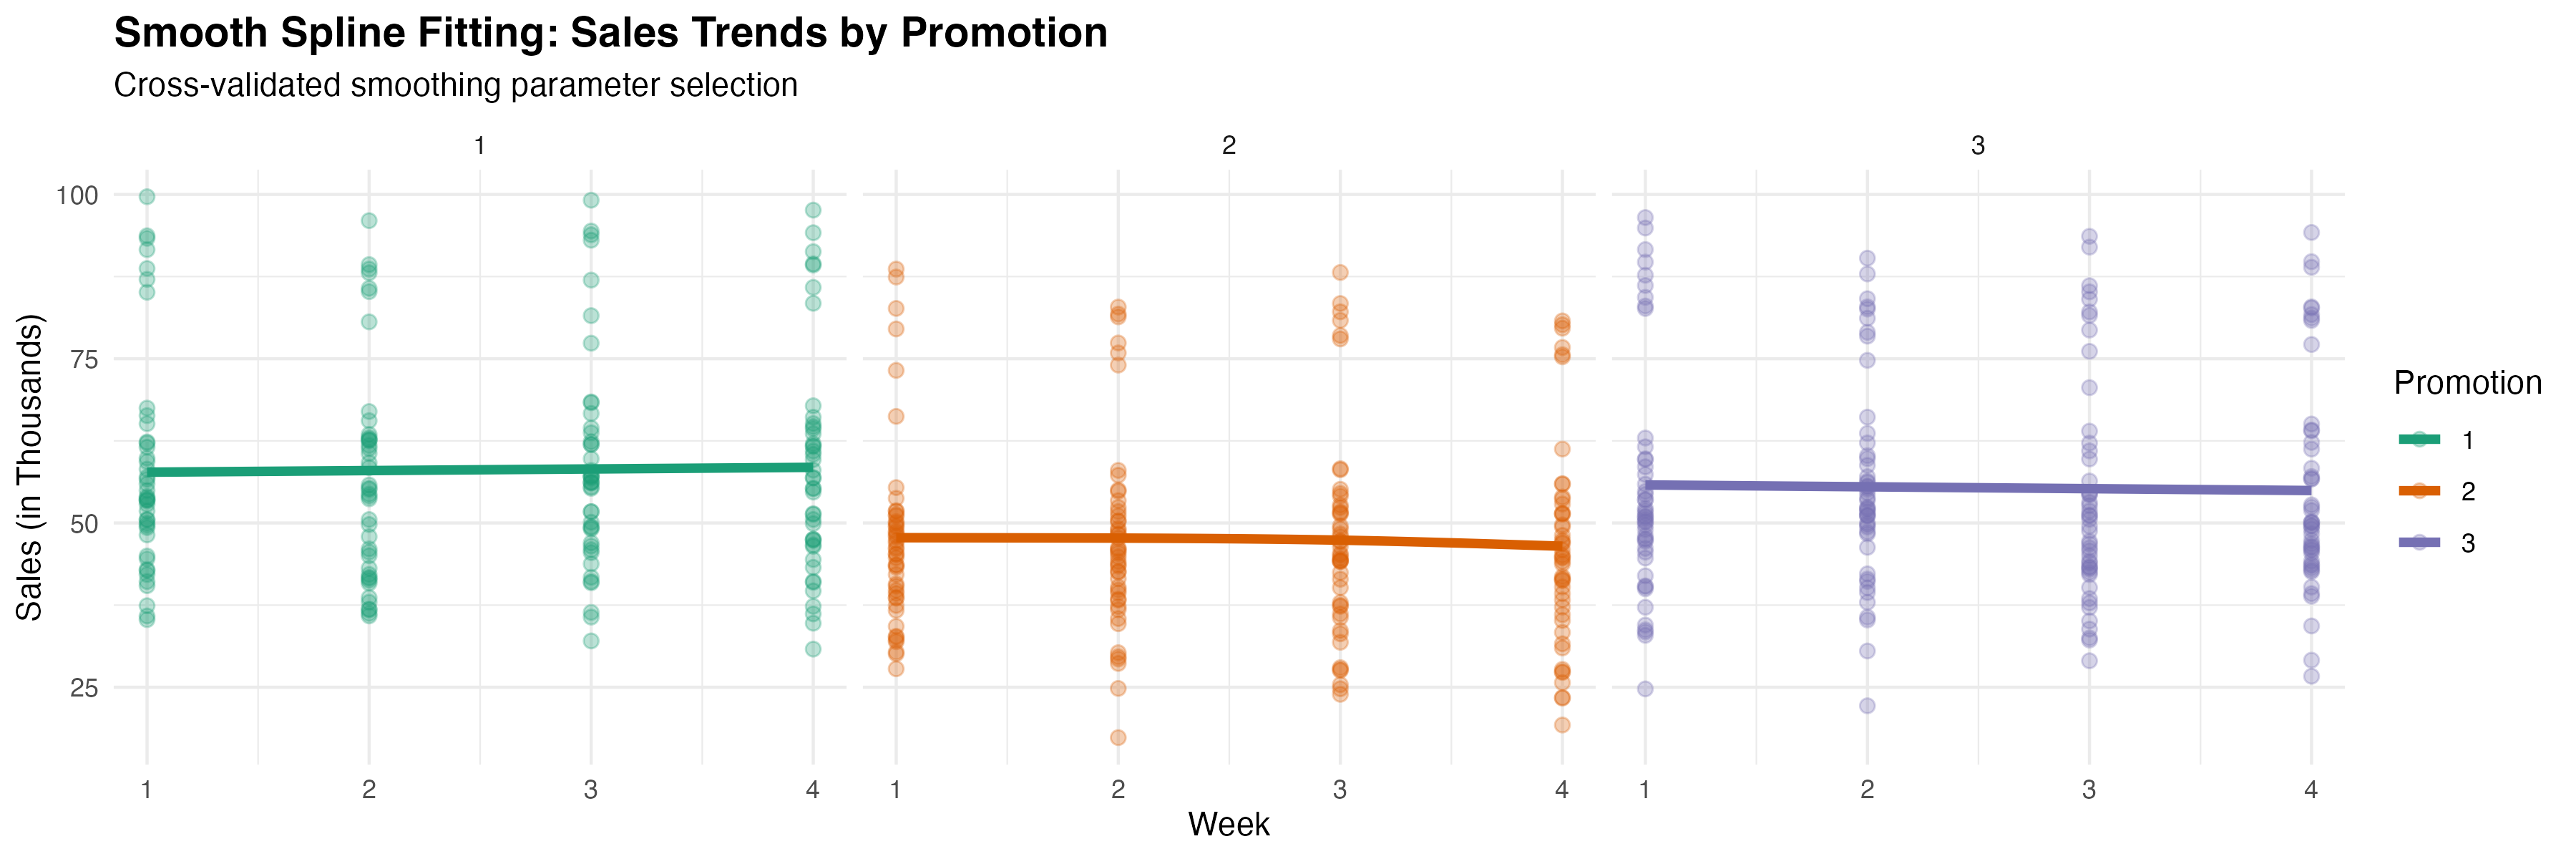
\includegraphics[width=\textwidth]{report_output/plot_splines.png}
\caption{Smooth Spline Fitting: Sales trends by promotion type. Cross-validated smoothing parameter selection ensures optimal bias-variance trade-off.}
\label{fig:splines}
\end{figure}

\subsubsection{Comparison of LOWESS and Smooth Splines}

Figure~\ref{fig:comparison} presents a side-by-side comparison of the two curve fitting methods, and Table~\ref{tab:model_comparison} summarizes the goodness-of-fit metrics.

\begin{figure}[H]
\centering
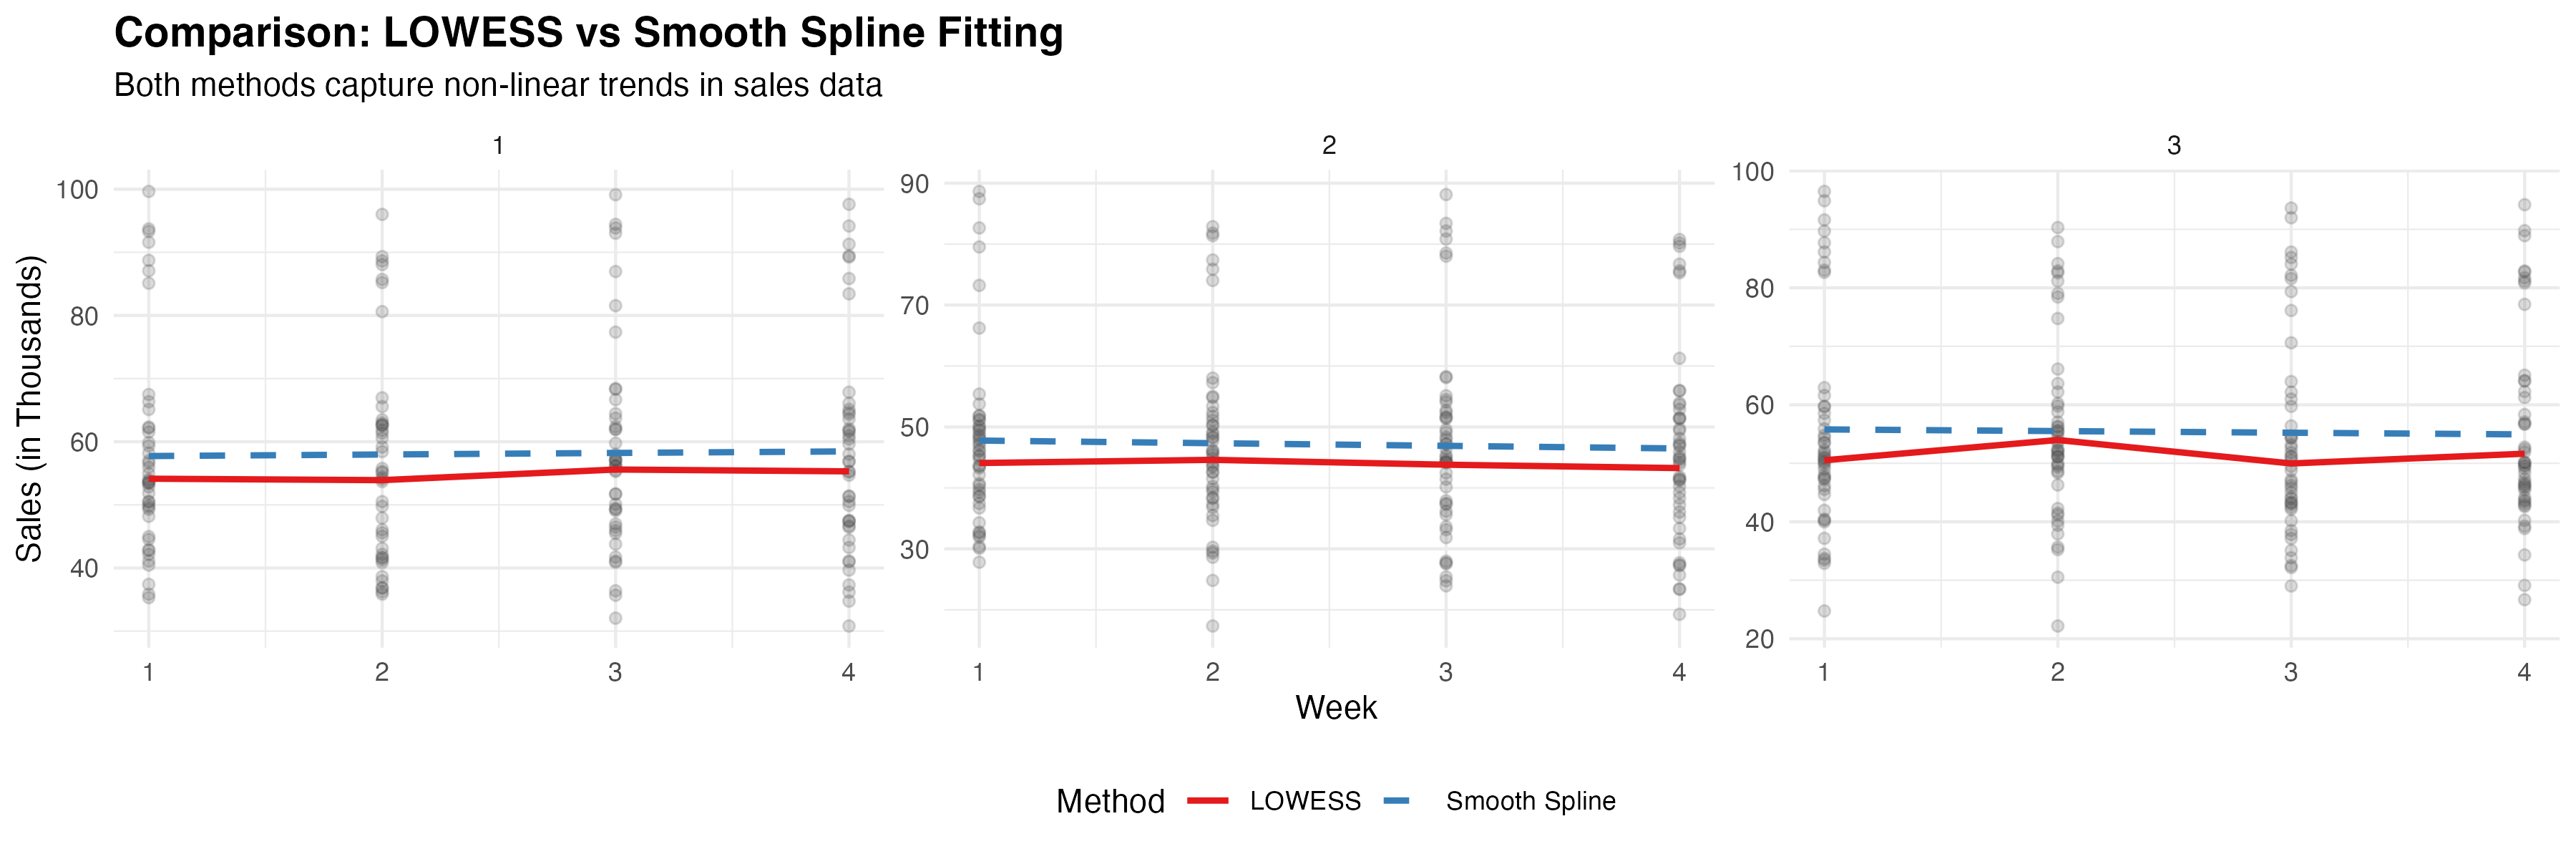
\includegraphics[width=\textwidth]{report_output/plot_comparison.png}
\caption{Comparison of LOWESS and Smooth Spline fitting methods. Both methods are overlaid on the raw data for each promotion type, illustrating differences in smoothing behavior.}
\label{fig:comparison}
\end{figure}

\begin{table}[H]
\centering
\caption{Model Comparison: Goodness-of-Fit Metrics by Promotion and Method}
\label{tab:model_comparison}
\begin{tabular}{llrrrrrr}
\toprule
\textbf{Promo} & \textbf{Method} & \textbf{RMSE} & \textbf{MAE} & \textbf{MAPE} & \textbf{$R^2$} & \textbf{AIC} & \textbf{BIC} \\
\midrule
1 & LOWESS & 16.8349 & 12.3886 & 20.94 & -0.0403 & 2147.38 & 3230.12 \\
1 & Spline & 16.5033 & 12.6602 & 22.71 & 0.0003 & 1456.54 & 1462.83 \\
2 & LOWESS & 15.4399 & 10.9145 & 23.63 & -0.0499 & 2314.62 & 3531.52 \\
2 & Spline & 15.0578 & 10.9040 & 25.40 & 0.0014 & 1558.90 & 1568.13 \\
3 & LOWESS & 17.1887 & 12.3753 & 22.09 & -0.0567 & 2354.96 & 3571.86 \\
3 & Spline & 16.7186 & 13.0183 & 24.99 & 0.0004 & 1596.53 & 1603.01 \\

\bottomrule
\end{tabular}
\end{table}

\subsection{Cross-Validation Results}

Leave-one-out cross-validation (LOOCV) was performed to assess the out-of-sample predictive accuracy of both methods. Table~\ref{tab:cv_results} presents the CV-RMSE and CV-MAE for each promotion and method.

\begin{table}[H]
\centering
\caption{Leave-One-Out Cross-Validation Results}
\label{tab:cv_results}
\begin{tabular}{llrr}
\toprule
\textbf{Promotion} & \textbf{Method} & \textbf{CV-RMSE} & \textbf{CV-MAE} \\
\midrule
1 & LOWESS & 17.1499 & 12.7043 \\
1 & Spline & 16.6998 & 12.8095 \\
2 & LOWESS & 15.6308 & 11.1369 \\
2 & Spline & 15.2220 & 11.0228 \\
3 & LOWESS & 17.5394 & 12.6906 \\
3 & Spline & 16.9025 & 13.1599 \\

\bottomrule
\end{tabular}
\end{table}

\subsection{Model Predictions}

Using the selected model, predictions were generated for weeks 1 through 6 (at 0.5-week intervals) for each promotion type. Figure~\ref{fig:predictions} shows the predicted sales trajectories alongside the observed data, with dotted vertical lines indicating the boundary of the original data range (weeks 1--4) beyond which predictions constitute extrapolations.

\begin{figure}[H]
\centering
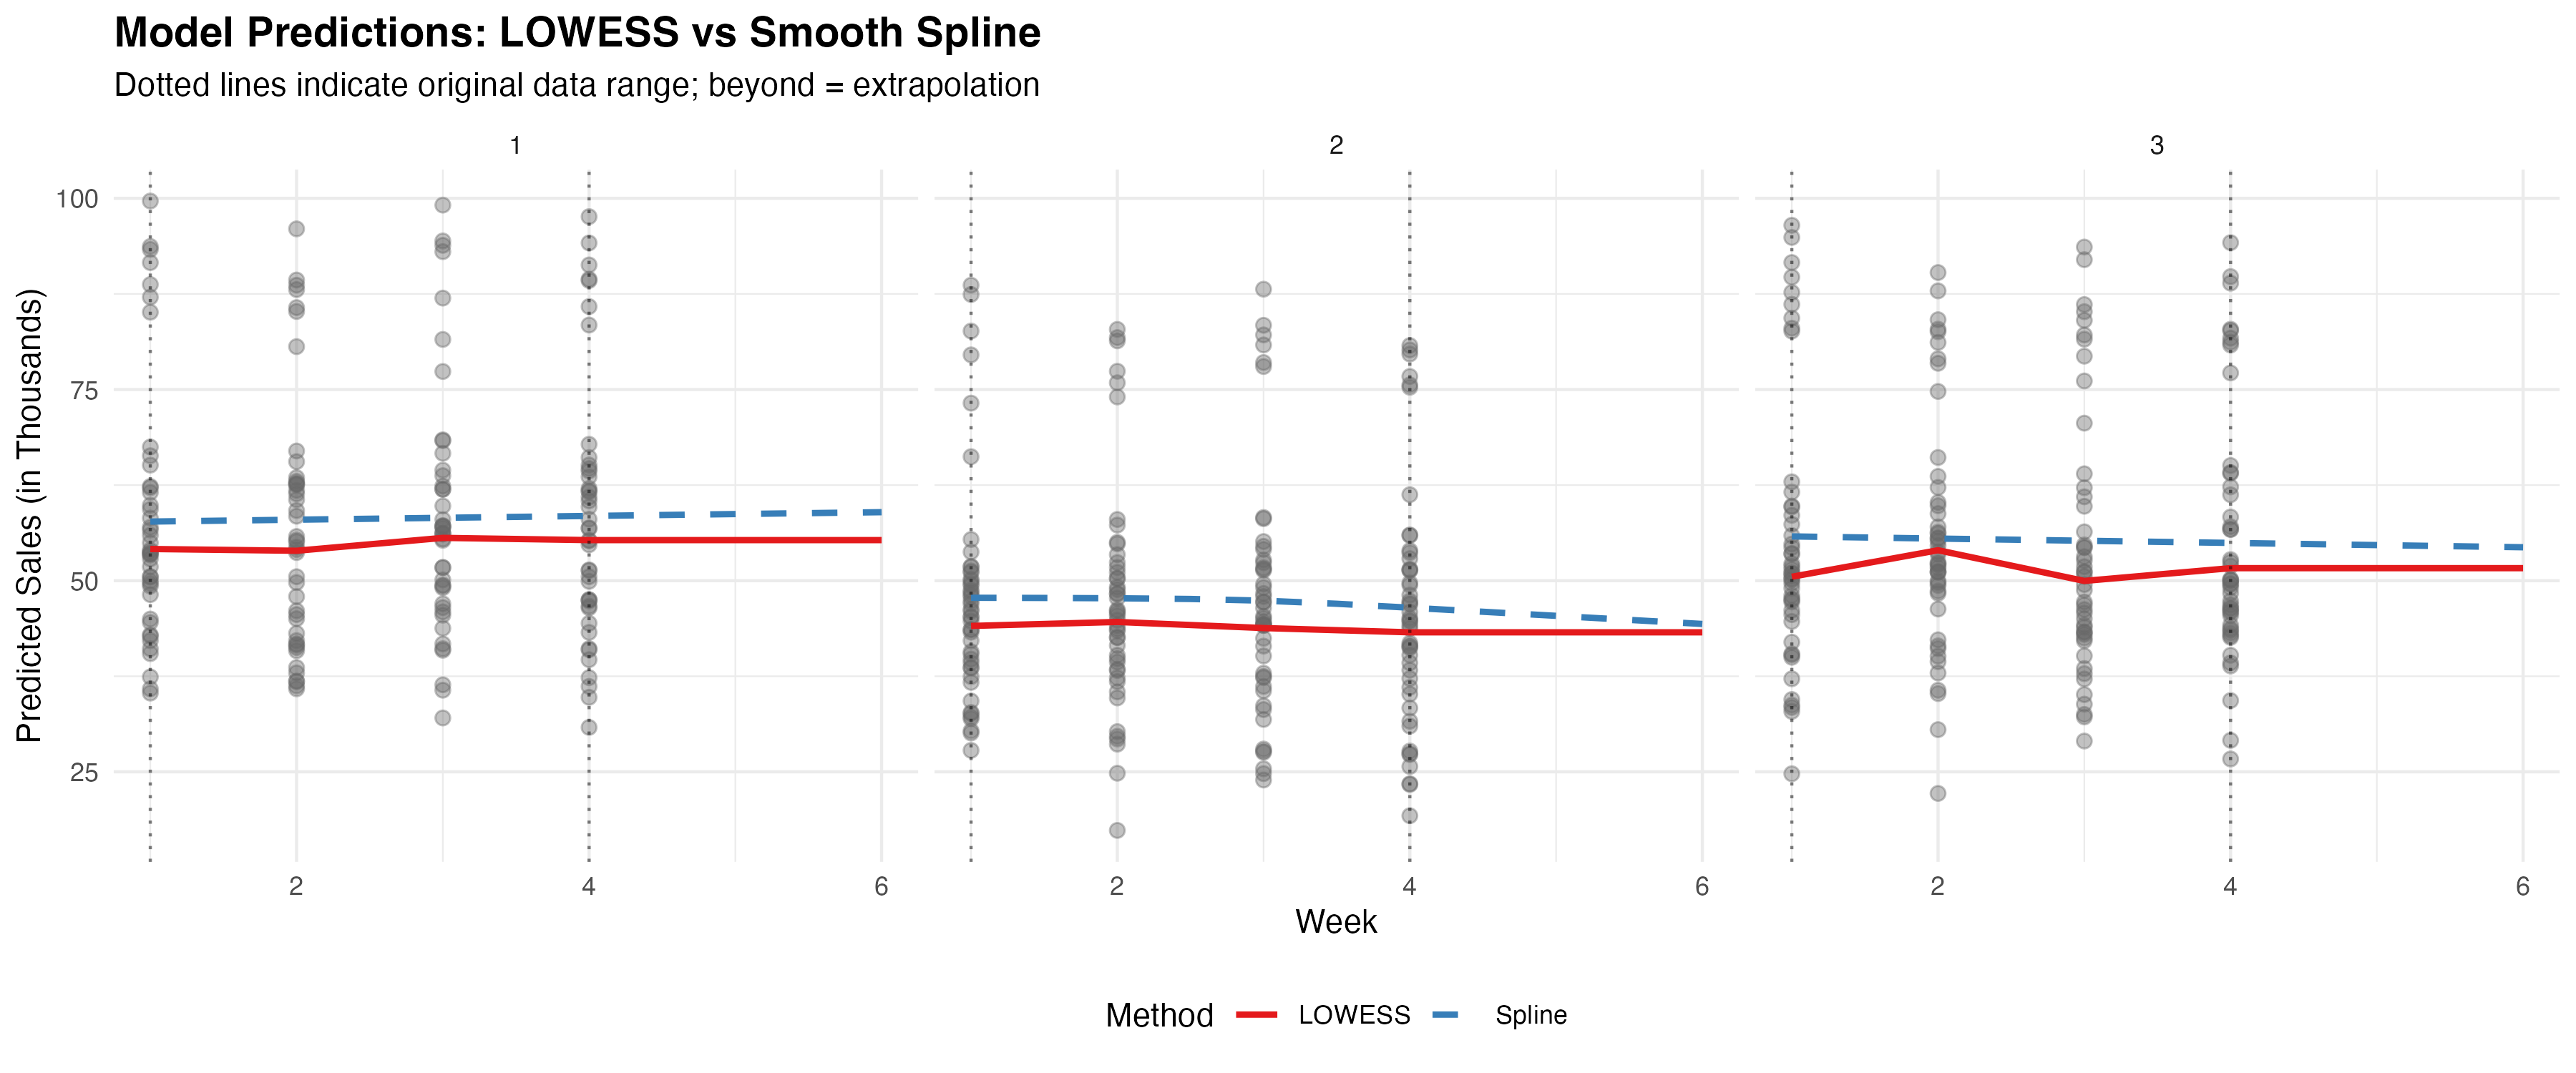
\includegraphics[width=\textwidth]{report_output/prediction_comparison.png}
\caption{Model Predictions: LOWESS vs Smooth Spline. Dotted vertical lines indicate the original data range; predictions beyond week 4 are extrapolations and should be interpreted with caution.}
\label{fig:predictions}
\end{figure}

\newpage

% ========== DISCUSSION ==========
\section{Discussion}

\subsection{Summary of Findings}

This study applied a comprehensive suite of non-parametric statistical methods to evaluate three marketing promotion strategies across 137 fast food store locations. The Kruskal-Wallis H-test detected statistically significant differences among the three promotion groups, confirming that not all promotions perform equally. Post-hoc Wilcoxon-Mann-Whitney U tests with both Bonferroni and Holm corrections identified the specific pairs of promotions that differ significantly in their sales outcomes. Median-based directional analyses quantified the practical magnitude of these differences in terms of both absolute sales differences and percentage changes.

The non-parametric curve fitting analysis demonstrated that both LOWESS and smooth splines adequately capture the temporal sales trends within each promotion group. The comparison of goodness-of-fit metrics and cross-validation results provided a principled basis for selecting between the two smoothing methods. The LOOCV procedure, in particular, offered an unbiased estimate of predictive performance by systematically evaluating each method's ability to predict unseen observations.

\subsection{Strengths and Limitations}

\textbf{Strengths:}
\begin{itemize}
    \item The use of non-parametric methods avoids distributional assumptions that may not hold for sales data, providing more robust inference.
    \item Multiple testing corrections (both Bonferroni and Holm) were applied to control the family-wise error rate, reducing the risk of false positive findings.
    \item Two complementary curve fitting methods were compared using multiple metrics and cross-validation, providing a thorough model evaluation.
    \item The analysis is fully reproducible, with all code available in the project repository.
\end{itemize}

\textbf{Limitations:}
\begin{itemize}
    \item The observation period is limited to four weeks, constraining the ability to detect longer-term promotional effects or seasonal patterns.
    \item The dataset does not include a control group (no promotion), so we can only compare promotions relative to each other rather than to a baseline.
    \item Store-level clustering (repeated measures across weeks within stores) is not explicitly modeled; observations from the same store may be correlated.
    \item LOWESS and smooth splines are primarily interpolation tools; extrapolation beyond the observed data range (weeks 5--6) should be interpreted cautiously.
    \item The analysis does not adjust for potential confounders such as market size and store age in the non-parametric tests, which could influence sales outcomes independently of promotion type.
\end{itemize}

\subsection{Suggestions for Future Research}

Future studies could address these limitations through several extensions:
\begin{itemize}
    \item Extending the observation period to capture longer-term and seasonal effects of promotional strategies.
    \item Incorporating mixed-effects or hierarchical models to account for the nested structure (weeks within stores, stores within markets).
    \item Stratifying the Kruskal-Wallis analysis by market size to examine whether promotional effectiveness varies across market segments.
    \item Including additional covariates such as store traffic, competitor proximity, and demographic characteristics.
    \item Comparing the non-parametric approaches with parametric alternatives (e.g., linear mixed models) to assess sensitivity of conclusions to modeling assumptions.
\end{itemize}

\newpage

% ========== REFERENCES ==========
\section*{References}
\addcontentsline{toc}{section}{References}

\begin{thebibliography}{9}

\bibitem{cleveland1979}
Cleveland, W. S. (1979). Robust locally weighted regression and smoothing scatterplots. \textit{Journal of the American Statistical Association}, 74(368), 829--836.

\bibitem{conover1999}
Conover, W. J. (1999). \textit{Practical Nonparametric Statistics} (3rd ed.). John Wiley \& Sons.

\bibitem{holm1979}
Holm, S. (1979). A simple sequentially rejective multiple test procedure. \textit{Scandinavian Journal of Statistics}, 6(2), 65--70.

\bibitem{kohavi2009}
Kohavi, R., Longbotham, R., Sommerfield, D., \& Henne, R. M. (2009). Controlled experiments on the web: Survey and practical guide. \textit{Data Mining and Knowledge Discovery}, 18(1), 140--181.

\bibitem{kruskal1952}
Kruskal, W. H., \& Wallis, W. A. (1952). Use of ranks in one-criterion variance analysis. \textit{Journal of the American Statistical Association}, 47(260), 583--621.

\bibitem{mann1947}
Mann, H. B., \& Whitney, D. R. (1947). On a test of whether one of two random variables is stochastically larger than the other. \textit{The Annals of Mathematical Statistics}, 18(1), 50--60.

\bibitem{wahba1990}
Wahba, G. (1990). \textit{Spline Models for Observational Data}. SIAM.

\end{thebibliography}

\end{document}
